% ======================= CHAPTER IV =======================
\chapter{Results}\label{ch:results}

\section{Hardware Developement}

El hardware del sistema de comunicación TTE, el cual fue bautizado como MAGIC \textit{(MAGnetic Induction Communication)} fue diseñado y construido para cumplir con un conjunto específico de requisitos y restricciones.
En primer lugar el sistema debe ser capaz de satisfacer la prueba de concepto logrando comunicación a una diatancia media pero significativa en un entorno subterráneo.
Asismismo el equipo no debe ser extremadamente voluminoso o pesado para facilitar su transporte y versatilidad en su uso.
\newp
The communication system is defined primarly by the magnetic coupling principe between two resonant coils, one used as transmitter and the other as receiver. Also the system has to be bidirectional, so both coils can work as transmitter or receiver depending on the comunication direction.
\subsection{Design}

El sistema de comunicación TTE está compuesto por varios elementos que trabajan en conjunto para lograr la transmisión y recepción de datos mediante inducción magnética.
El elemento principal es la bobina resonante, la cual está diseñada para generar y recibir campos magnéticos en una frecuencia específica. Además de la bobina, 
el sistema incluye un amplificador para aumentar la potencia del mensaje transmitido y un sistema de switching para intercambiar la conexión de la bobina resonante entre los canales de entrada y salida del sistema, dependiendo de la dirección de comunicación deseada (TX o RX).
\newp
Here is a conceptual diagram of the complete system in figure \ref{fig:system-diagram}.

\begin{figure}[H]
    \centering
    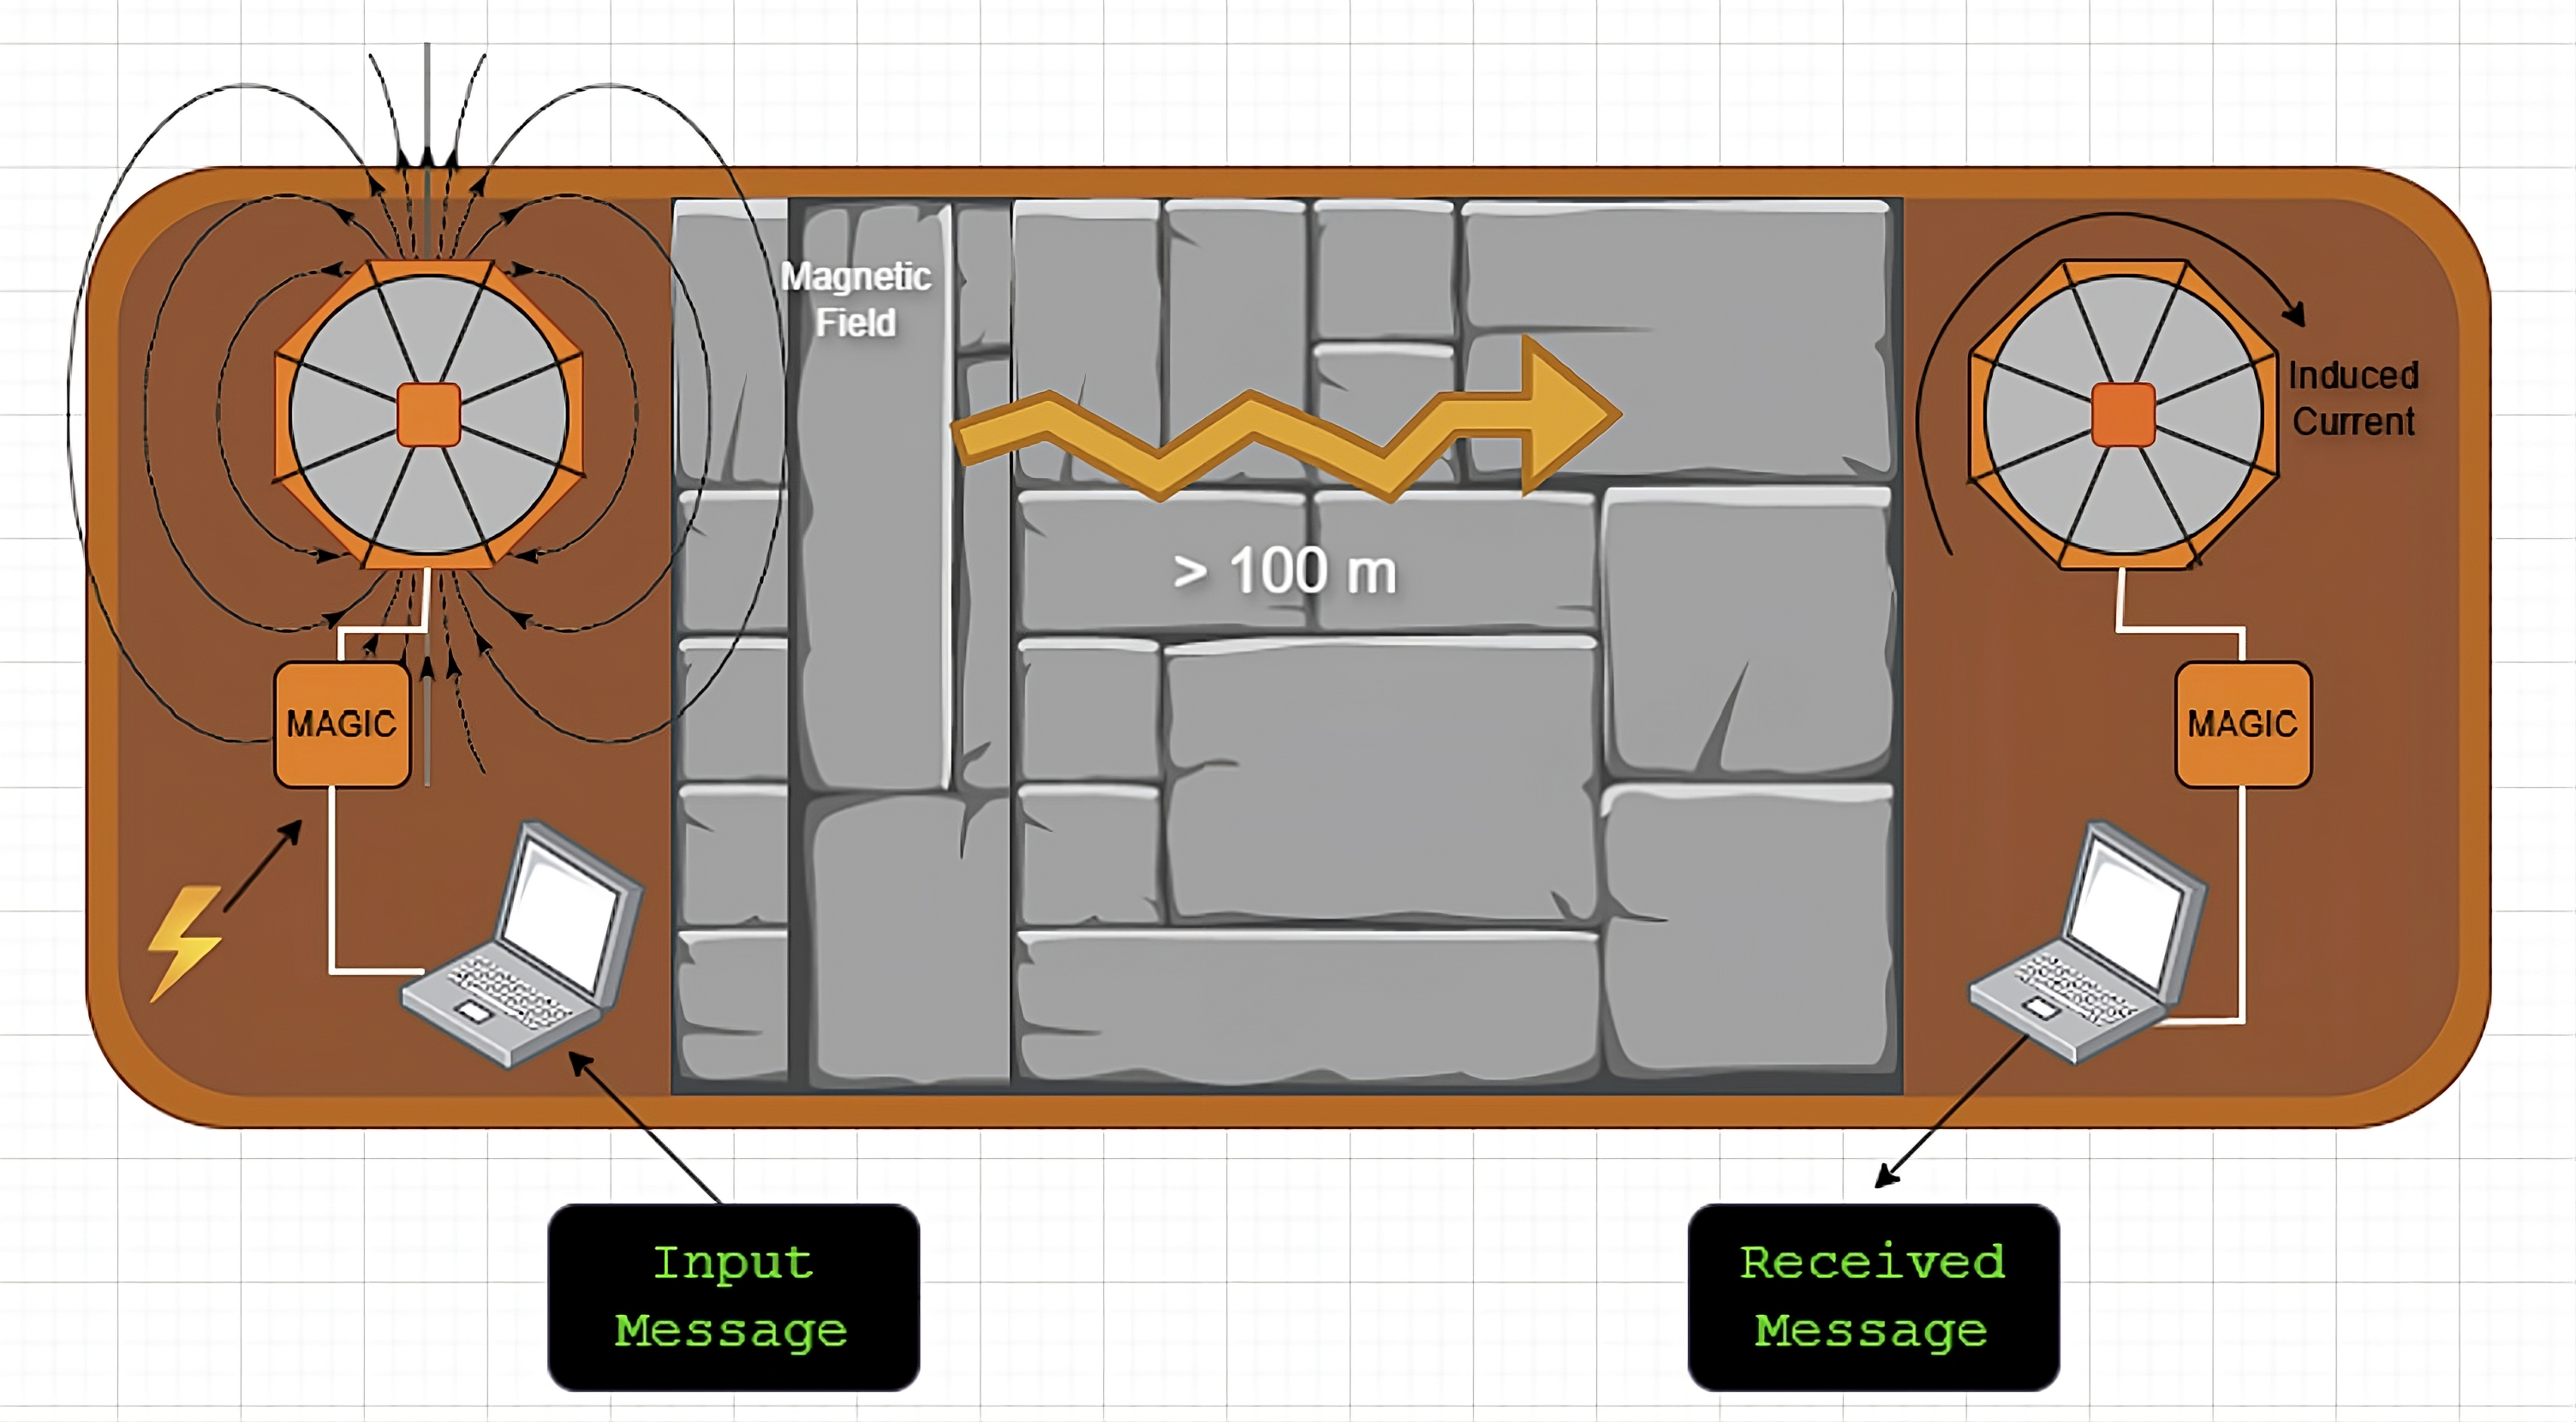
\includegraphics[width=0.8\textwidth]{img/esquema_blanco.png}
    \caption{Conceptual diagram of the complete TTE communication system.}
    \label{fig:system-diagram}

\end{figure}

As shown in the diagram, we can start from left to right with the generation of a text message, wich is codificated and modulated digitally in a computer. Then the digital signal is converted to analog using a DAC, this signal is amplified using a class D audio amplifier to drive the resonant coil. The flux of current at the coil generates a variable magnetic field, as equation \ref{equation_of_ampere_maxwell} describes in section 2. This variable magnetic field, that is centered at a pretty low frequency (VLF band of radio), propagates through the environment, penetrating rock soil and solid material and reaching the receiving coil.
\newp
The magnetic flux that pass perpendicularly through the coil structure can induce a voltage in bornes of the receiving coil, according to Faraday's law of induction \ref{equation_of_magnetic_induction}. This signal can be digitalized using an ADC, demodulated, decoded and corrected in a computer to recover the original text message.
\newp
To answer a received message, the same process is followed in reverse thanks to the switching circuit.
\newp
The schematic diagram of the system is shown in figure \ref{fig:system-schematic}.

\begin{figure}[H]
    \centering
    \includegraphics[width=1\textwidth]{img/schematic.png}
    \caption{Schematic diagram of the complete TTE communication system.}
    \label{fig:system-schematic}
\end{figure}

As is shown in figure \ref{fig:system-schematic}, the system is composed by the following main blocks: Coil (1), Battery (2), USB audio Interface (3) and the core module that contains the Amplifier, a ground loop isolator and the switching Switching circuit(rest of diagram).
\subsection{Coil}
La bobina resonante corresponde a al elemento encargado de transmitir el campo magnético variable al circular corriente por su estrcutura (Transmisor) y de entregar la fem inducida en presencia al atravesar por su estructira las líneas de campo magnético transmitido (Receptor). En vista de lograr el objetivo de comunicación a distancia significativa, la bobina debe ser diseñada para maximizar la eficiencia de la transferencia de energía magnética entre el transmisor y el receptor, es por esto que se optó en primera instancia por un diseño simple toroidal, donde las variables de diseño y construcción se reducen a número de vueltas $N$, diámetro de la estructura $D$, y el calibre del conductor $C$.
\newp
Para esta primera versión se fijó el diámetro de la bobina en 55 cm, ya que correspondía a un tamaño manejable y portátil. El calibre del conductor se seleccionó en función de su costo, resistencia eléctrica y peso, optando por un cable de cobre esmaltado de 17 AWG. A continuación se muestra una tabla de resistencia eléctrica en función del calibre del conductor, entregada por el fabricante.

\begin{table}[H]
    \centering
    \begin{tabular}{|c|c|c|}
    \hline
    \textbf{Calibre (AWG)} & \textbf{Diámetro (mm)} & \textbf{Resistencia (ohm/m)} \\ \hline
    10                     & 2.588                  & 0.00328                      \\ \hline
    12                     & 2.053                  & 0.00521                      \\ \hline
    14                     & 1.628                  & 0.00829                      \\ \hline
    16                     & 1.291                  & 0.01317                      \\ \hline
    17                     & 1.150                  & 0.01660                      \\ \hline
    18                     & 1.024                  & 0.02100                      \\ \hline
    20                     & 0.812                  & 0.03340                      \\ \hline
    \end{tabular}
    \caption{Resistencia eléctrica en función del calibre del conductor.}
    \label{tab:resistance-table}
\end{table}
%Ajustar valores segun tabla real.

De esta manera al escoger tal calibre, el cual corresponde a 1.15 mm de diámetro y considerando una masa total cercana a los $1.5 Kg$, se logra una extensión total de 156 metros, lo que se traduce en $N=90$, con esta extensión la resistencia total de la bobina resulta en 2.6 ohmios. Sin embargo al ser medida de forma experimental el valor de resistencia total es de $3 \Omega$, un valor ideal considerando la resistencia a la cual opera el amplificador clase D seleccionado para el proyecto.
\newp
Ya definida la geometría y características de la bobina, se procede a calcular los parámetros eléctricos asociados a la misma. En primera instancia se calcula la inductancia de la bobina utilizando la fórmula para una bobina toroidal:
\begin{equation}
    L = \frac{\mu N^2 A}{l}  %%Comprobar
\end{equation}
Donde:
\begin{itemize}
    \item $L$ es la inductancia en Henrios (H).
    \item $\mu$ es la permeabilidad del núcleo (para aire, $\mu_0 = 4\pi \times 10^{-7} H/m$).
    \item $N$ es el número de vueltas.
    \item $A$ es el área de la sección transversal del toroide en metros cuadrados ($m^2$).
    \item $l$ es la longitud media del camino magnético en metros (m).
\end{itemize}
Considerando un área de sección transversal aproximada de $A = 0.2375 m^2$ y una longitud media del camino magnético de $l = 1.7 m$, se obtiene una inductancia teórica de $L \approx  H$. Sin embargo, al medir la inductancia de la bobina construida utilizando un medidor LCR, se obtiene un valor experimental de $L_1 = 10.67  mH$ y $L_2 = 10.55 mH$. Esta discrepancia puede atribuirse a factores como la distribución no uniforme del campo magnético, las pérdidas en el conductor y las tolerancias en la construcción de la bobina.
\newp
Finalmente, se calcula la capacitancia necesaria para sintonizar la bobina a la frecuencia de resonancia deseada, que en este caso es de 3.2 kHz. La frecuencia de resonancia $f_0$ de un circuito LC está dada por la fórmula:
\begin{equation}
    f_0 = \frac{1}{2\pi \sqrt{LC}}
\end{equation}
Despejando para la capacitancia $C$, se obtiene:
\begin{equation}
    C = \frac{1}{(2\pi f_0)^2 L}
\end{equation}

De esta menera la capacitancia necesaria para sintonizar la bobina a $\approx 3.2 kHz$ resulta en $C \approx 237 \mu F$ para $L_1$ y $C \approx 240 \mu F$ para $L_2$. Se seleccionaron capacitores cerámicos de 470 $\mu F$  dispuesto en serie para alcanzar el valor deseado, considerando la tolerancia de los componentes. A continuación se muestra una figura de la bobina construida:

\begin{figure}[H]
    \centering
    \includegraphics[width=0.5\textwidth]{img/coil.png}
    \caption{Bobina resonante construida para el sistema TTE.}
    \label{fig:coil}
\end{figure}

Al medir la función de transferencia para en un sistema donde se tiene una de las bobinas sintonizadas y otra más pequeña sin sintonizar puede observarse en la figura \ref{fig:transfer-function} para $L_1$ y $L_2$ que la frecuencia de resonancia se encuentra cercana a los 3.2 kHz, cumpliendo con el diseño inicial.
\begin{figure}[H]
    \centering
    \includegraphics[width=1\textwidth]{img/TF_L1_L2.png}
    \caption{Función de transferencia del sistema de bobinas resonantes.}
    \label{fig:transfer-function}
\end{figure}

Se muestra a continuación la función de transferencia del sistema completo (end-to-end) medido a una distancia de 2 metros entre las bobinas.

\begin{figure}[H]
    \centering
    \begin{subfigure}[b]{0.49\textwidth}
        \centering
        \includegraphics[width=\textwidth]{img/Desfase_end_2_end_2.jpg}
        \caption{Phase shift}
        \label{fig:sub2-transfer-function-system}
    \end{subfigure}
    \hfill
    \begin{subfigure}[b]{0.49\textwidth}
        \centering
        \includegraphics[width=\textwidth]{img/Relacion_de_potencia_end_2_end_3.jpg}
        \caption{Power relation}
        \label{fig:sub1-transfer-function-system}
    \end{subfigure}
    \caption{Transfer function of complete system at 2 meters distance.}
    \label{fig:transfer-function-system}
\end{figure}


If we review particularly the power relation graph in figure \ref{fig:sub1-transfer-function-system} we can observe that the maximum power transfer occurs at a frequency of approximately 3.2 kHz, specifically at 3150 Hz, at this point we have an approximaly analog bandwidth of ~450 Hz considering a decaiment of 3 dB from center frequency. Here it's a zoom of this graph in figure \ref{fig:zoom-transfer-function-system}.

\begin{figure}[H]
    \centering
    \includegraphics[width=0.7\textwidth]{img/bw end-2-end.png}
    \caption{Bandwidth available for end-to-end system at 2 meters distance.}
    \label{fig:zoom-transfer-function-system}

\end{figure}

If we consider this geometry and values of the coil, we can estimate the magnetic field generated at the center of the coil using the formula decribed on section 2 \ref{equation_of_magnetic_field} for the magnetic field at the center of a circular loop:








\subsection{Amplifier and GLI}

The amplifier choosed for the application corresponds to a class D Power Amplifier Board XH-M544  based on the Texas Instruments chips TPA3116D2 and NE5532. This amplifier is capable of delivering a maximum power of 150W Mono, considering a voltage of 26 V.

\newp
This component was selected due to its ability to deliver high power output with high efficiency, which is crucial for driving the resonant coil effectively. The amplifier operates in class D mode, which means it uses pulse-width modulation (PWM) to amplify the input signal, resulting in lower heat dissipation and improved energy efficiency compared to traditional linear amplifiers. %ref pendiente.
Also as was mentioned before, the system will operate in a frequency range around 3.2 kHz, within the audible spectrum. Here is a figure of the amplifier used:

\begin{figure}[H]
    \centering
    \includegraphics[width=0.5\textwidth]{img/amp.png}
    \caption{Amplificador de audio clase D TPA3116D2.}
    \label{fig:amplifier}
\end{figure}

The input signal to the amplifier is provided by a USB audio interface, and this signal is isolated from ground loops using a Ground Loop Isolator (GLI). The GLI is essential to prevent unwanted noise and hum that can be introduced into the audio signal due to differences in ground potential between the computer and the amplifier. By isolating the audio signal, the GLI helps maintain signal integrity and ensures that the transmitted message is clear and free from interference.
%is neccesary if now we utilize a battery?
\newp
Here is a schematic diagram of the GLI used in MAGIC:

\begin{figure}[H]
    \centering
    \includegraphics[width=0.6\textwidth]{img/GLI.png}
    \caption{Schematic diagram of the Ground Loop Isolator (GLI).}
    \label{fig:gli-schematic}
\end{figure}

\subsection{Switching Circuit}
The switching circuit is essential for enabling bidirectional communication in the TTE system, for this prototype this function is supplied by a positional selector, that means, mannually.
\newp
Here is a schematic diagram of the positional selector used MAGIC:.
\begin{figure}[H]
    \centering
    \includegraphics[width=0.8\textwidth]{img/selector.png}
    \caption{Schematic diagram of the switching circuit.}
    \label{fig:switching-circuit}

\end{figure}

This device conmute the bornes of the resonant coil between the amplifier output (TX mode) and the audio interface input (RX mode). When the selector is in position 1, the coil is connected to the amplifier output, allowing it to transmit signals. Conversely, when the selector is in position 2, the coil is connected to the audio interface input, enabling it to receive signals. Also the selector at TX mode allows the amplifier to be powered on.

 

\subsection{Audio Interface}

The audio interface selected for the TTE communication system is the SoundBlaster Play! 3 by Creative Labs. This USB audio interface is chosen for its high-quality audio conversion capabilities, compact size, input and output separately channel and ease of use. In terms of USB audio interfaces, the SoundBlaster Play! was the best option available considering cost and Portability.
\newp
Here is a figure of the audio interface used:
\begin{figure}[H]
    \centering
    \includegraphics[width=0.3\textwidth]{img/sbp3.png}
    \caption{USB Audio Interface SoundBlaster Play! 3.}
    \label{fig:audio-interface}
\end{figure}


\section{Software Developement}
\subsection{Modulation system}
\subsubsection{Non-coherent FSK}
 The detection system works as a typical non-coherent FSK receiver. 
The incoming signal is filtered at the beggining to reduce the noise influence in terms os  operations in the time domain.
%is there any best way of describing this? What are the others benefits of filtering the signas with a digital bandpassfilter,if are any ?
\newp
Why a Non coherent FSK system?
The non-coherent FSK system is selected due to its robustness to phase variations and frequency offsets %(Include bibiliography about this) 
In comparisson for example models based on PSK or QAM, that are more sensitive to phase noise and frequency offsets. FSK modulation allows the receiver to detect the transmitted symbols based on energy detection in specific frequency bands, without requiring precise phase synchronization. This characteristic makes non-coherent FSK particularly suitable for TTE communication systems, where the channel conditions can be highly variable and unpredictable.
Here is a diagram of the non-coherent FSK modulation and demodulation process in Figure \ref{fig:fsk-mod-demod}.

\begin{figure}[H]
    \centering
    \includegraphics[width=0.8\textwidth]{img/Diagrama_Receptor.png}
    \caption{Block diagram of the non-coherent FSK modulation and demodulation process.}
    \label{fig:fsk-mod-demod}
\end{figure}

As I mentiones brewly the last paragraph, at the beggining the digital signal in filtered and then passes to a Window of len N, that is an important number, the dimensions of this Window
determine the cost of the processing process, that's because the bigger the window is, the main process that's comes right after is the correlation.

\subsubsection{Correlation Process}

Correlation is a mathematical operation that measures the similarity between two signals as a function of the time-lag applied to one of them %Include Bibliography. 
In the context of signal processing, correlation is often used to detect the presence of a known signal (template) within a received signal that may be corrupted by noise.
In the non-coherent FSK detection system, the correlation process is used to compare the received signal with predefined reference signals corresponding to each of the FSK frequencies. 
The correlation here is performs between the received signal (or a portion of it) and a known preamble.
This preamble is a specific sequence of symbols that is transmitted at the beginning of each data packet. The purpose of the preamble is to help the receiver synchronize with the incoming signal and accurately detect the start of the data transmission. %Include Reference)
Here we have several main design parameters: an optimar lenght of preamble, its structure, and optimal use of our computation resources, thats because as bigger the lenght of correlation inputs, more calculus to do in each earing time. %Improve redaction
The size of the window is key of the times that the function \textit{Correlation by parts} is called. 
The output of the correlation process is a correlation coefficient that indicates the degree of similarity between the received signal and the reference signal at different time lags. A high correlation coefficient at a specific time lag suggests that the known signal is present in the received signal at that time.
% Include bibliography
The correlation formula (\ref{eq:Correlation_dig}), given in previous chapter, is used as a the main operation of correlation IQ System.



\subsubsection{Correlation by parts algorithm}

The correlation by parts algorithm is a method to efficiently compute the correlation between a received signal and the known parts of the preamble considering the similarity with in phase and cuadrature tones.
\newp
At the beggining we have a window of size $N_w$, wich is the size of the total preamble ($N_symbols$ multiplied by the size of each symbol $M$), plus the amount of samples incoming in an earing cicle ($N_c$). With this structure we allow only one instance of correlation where the incoming preamble is fully contained in the window. So from the window we can define $N_symbols$ parts, where each part $S_N$ corresponds to the section that could contain te $``N"th$ symbol of the preamble.
\newp
once we have the $S_N$ and $P_N$ (the $``N"th$ symbol of the preamble) we can compute the correlation between them using the formula (\ref{eq:Correlation_dig}). That is implemented as the scipy function \textit{correlate} with mode ``valid", that has an output size of the difference between the two arguments ($S_N - P_N$). For each of these $``N"$ calculus The $S_N$ signals are correlated with its corresponding $P_N$ symbol of and its version in cuadrature, that means the following:

\begin{equation}
\label{eq:corr_IQ}
\begin{split}
    I_{N} &= \sum_{k=0}^{M-1} S_{N}[k] \sin(2 \pi f_{N} k T_s) \\
    Q_{N} &= \sum_{k=0}^{M-1} S_{N}[k] \cos(2 \pi f_{N} k T_s)
\end{split}
\end{equation}

where $f_N$ is the frequency of the $``N"th$ symbol of the preamble and $T_s$ is the sampling period.
\newp

So at the output we have two arrays that represents the similarity of the incoming signal section with the correspondig symbol in phase and cuadrature. If we consider the totallity of operations we can define two Matrix I and Q of size $N_symbols$ x $n_c$, where each row corresponds to the arrays resulted in \ref{eq:corr_IQ}:

\begin{equation}
\label{eq:matrix_IQ}
    I = \begin{bmatrix}
    I_{1}[0] & I_{1}[1] & \dots & I_{1}[n_c-1] \\
    I_{2}[0] & I_{2}[1] & \dots & I_{2}[n_c-1] \\
    \vdots & \vdots & \ddots & \vdots \\
    I_{N}[0] & I_{N}[1] & \dots & I_{N}[n_c-1]
    \end{bmatrix}, \quad
    Q = \begin{bmatrix}
    Q_{1}[0] & Q_{1}[1] & \dots & Q_{1}[n_c-1] \\
    Q_{2}[0] & Q_{2}[1] & \dots & Q_{2}[n_c-1] \\
    \vdots & \vdots & \ddots & \vdots \\
    Q_{N}[0] & Q_{N}[1] & \dots & Q_{N}[n_c-1]
    \end{bmatrix}
\end{equation}

Then we take the absolut value of each element of the two matrix and sum them to obtain a final correlation matrix C:

\begin{equation}
\label{eq:final_correlation_matrix}
    C = \begin{bmatrix}
    |I_{1}[0]| + |Q_{1}[0]| & |I_{1}[1]| + |Q_{1}[1]| & \dots & |I_{1}[n_c-1]| + |Q_{1}[n_c-1]| \\
    |I_{2}[0]| + |Q_{2}[0]| & |I_{2}[1]| + |Q_{2}[1]| & \dots & |I_{2}[n_c-1]| + |Q_{2}[n_c-1]| \\
    \vdots & \vdots & \ddots & \vdots \\
    |I_{N}[0]| + |Q_{N}[0]| & |I_{N}[1]| + |Q_{N}[1]| & \dots & |I_{N}[n_c-1]| + |Q_{N}[n_c-1]|
    \end{bmatrix}
\end{equation}

So in the components of this last matrix we have a certain measure about similarity between the incoming signal sections and the preamble symbols, in every columns there is an intant of time so if we sum along the rows we can obtain a final correlation vector that indicates the total similarity between the incoming signal and the whole preamble at each instant of time:
\begin{equation}
\label{eq:final_correlation_vector}
    V = \begin{bmatrix}
    \sum_{n=1}^{N} C_{n}[0] & \sum_{n=1}^{N} C_{n}[1] & \dots & \sum_{n=1}^{N} C_{n}[n_c-1]
    \end{bmatrix}
\end{equation}

As result we can see something like this:

\begin{figure}[H]
    \centering
    \includegraphics[width=0.7\textwidth]{img/Simulacion corr IQ.png}
    \caption{Resulted Correlation by parts with 24 symbols preamble.}
    \label{fig:corr-by-parts-diagram}
\end{figure}

\subsubsection{Preamble design}

Tal y como se explicó en el diseño del sistema de recepción y detección del mensaje, el preámbulo juega un rol fundamental en la sincronización y posterior demodulación de los símbolos transmitidos. El preámbulo debe ser diseñado cuidadosamente para maximizar la probabilidad de detección en presencia de ruido y otras distorsiones del canal.
\newp
En este sentido se optó por una secuencia de símbolos aleatorios generada de forma computacional, la cual es conocida tanto por el transmisor como por el receptor. Esta secuencia debe ser lo suficientemente larga para proporcionar una referencia clara para la detección, pero no tan larga como para consumir un tiempo excesivo de transmisión.
\newp
Se definió entonces un largo total de 12 segundos de preámbulo. Este valor fue definido a partir de meses de pruebas a diferentes distancias de comunicación en entornos subterráneos, en tanto el peak de correlación fuese visible en las condiciones de comunicación objetivo del proyecto no había un límite para su extensión temporal. Este largo de preámbulo en particular es la consecuencia del trade off entre probabailidad de detección y un tiempo de transmisión aceptable para la aplicación.
\newp  
A continuación se muestran los resultados de correlación por partes para distintas estructuras de preámbulo considerando un largo total de 12 segundos.

\begin{figure}
    \centering
    \label{fig:preamble-corr-models}
    \includegraphics[width=1\textwidth]{img/Simulacion corr modelos_2.png}
    \caption{Correlation by parts for different preamble structures with 12 seconds length.}
\end{figure}

Some relevant data about this excersice is summarized in the following table:
\newp

\begin{tabular}{|l|l|l|l|l|l|l|}
\hline N & M & Max Peak & Std Noise & Mean Noise & Ratio & Time (s) \\
\hline 3 & 192000 & $4.00 \mathrm{e}+05$ & 4842.85 & 14029.95 & 16.86 & 0.81 \\
\hline 6 & 96000 & $4.04 \mathrm{e}+05$ & 6141.66 & 22835.93 & 11.5 & 1.47 \\
\hline 12 & 48000 & $4.19 \mathrm{e}+05$ & 4233.53 & 33777.56 & 9.91 & 2.58 \\
\hline 24 & 24000 & $4.09 \mathrm{e}+05$ & 5155.71 & 48747.34 & 6.92 & 5.71 \\
\hline 48 & 12000 & $4.05 \mathrm{e}+05$ & 4506.15 & 69383.46 & 5.17 & 13.72 \\
\hline
\end{tabular}

En la figura %\ref{fig:preamble-corr} 
se observa que si bien el nivel de correlación IQ es similar para cada topología de preámbulo considerada, a medida que se incrementa el número de símbolos  en la secuencia, el peak de correlación es más "delgado", es decir, se concentra en un menor número de instantes de earing. Esto es beneficioso para el sistema de detección, ya que permite una identificación más precisa del inicio del mensaje transmitido.

\subsubsection{Ortogonality and Bandwidth}

Tal y como se mencionó en capítulos anteriores, la ortogonalidad entre las portadoras es un aspecto crucial en los sistemas de modulación FSK, ya que garantiza que las señales transmitidas en diferentes frecuencias no interfieran entre sí, dicho de otra manera, la energía de un símbolo transmitido en una frecuencia determinada no entra en el canal espectral de un símbolo adyacente en cuanto a la constelación de símbolos.
/newp
Para que se cumpla la condición de ortogonalidad se debe considerar la relación entre la frecuencia de sampleo y la cantidad de muestras por símbolo, es decir el valor inverso de la duración temporal de cada símbolo. La relación entre las frecuencias de las portadoras $f_1$ y $f_2$ debe cumplir con la siguiente ecuación:

\begin{equation}
    f_2 - f_1 = \frac{k}{T_s} = \frac{k f_s}{N_s}
\end{equation}

En este caso, se tiene que la frecuencia de sampleo es de 48 kHz, y debe definirse la cantidad de muestras por símbolo $N_s$. Para determinar el valor óptimo de $N_s$, se realizaron diversas pruebas variando este parámetro y observando su impacto en la tasa de error de símbolos demodulados (SER) del sistema. A continuación se muestra la variación de SER en función del largo del símbolo para un valor de SNR definido, el cual corresponde al objetivo mínimo a lograr con el sistema de comunicación TTE, en este caso $SNR=-10 dB$ %detallar luego el criterio para cálculo de SNR (en la banda, qué banda) .

\begin{figure}[H]
    \centering
    \includegraphics[width=0.7\textwidth]{img/SER_vs_Ns.png}
    \caption{SER vs Ns for 8-FSK and 16-FSK at SNR = -10 dB.}
    \label{fig:SER-vs-Ns}
\end{figure}

Considerando un Bandwidth de 200 Hz se tiene que un largo de símbolo de 24000 es un valor ideal considerando modelos de 8 y 16 FSK, en este punto marcado con una línea punteada roja en la figura \ref{fig:SER-vs-Ns} muestra una tasa de error cercana al 12\% en el caso de 16 símbolos y 5\% en el caso de 8 símbolos. Para ambos modelos este nivel de error es aceptable considerando que posteriormente se incluirá un código de corrección de errores simple. Se opta por este largo de símbolo y no uno mayor que pudiese disminuir aún el SER debido a que no se desea sav¿crificar en demacía la tasa de datos el sistema, manteniendo un compromiso adecuado entre velocidad de transmisión y robustez frente al ruido.
\newp
De esta manera ya habiendo fijado el valor de $N_s=24000$, se procede a calcular la separación entre las frecuencias de las portadoras para cumplir con la condición de ortogonalidad. Considerando $k=1$ se tiene que la separación mínima entre las portadoras es de 2 Hz. Sin embargo, teniendo en cuenta que la resolución de la FFT en el demodulador depende de la cantidad de muestras por símbolo, se opta por seleccionar una separación mayor dejando canales espectrales sin utilizar para evitar interferencias entre símbolos adyacentes. Mas adelante se observará la diferencia de desempeño al considerar un modelo de demodulación single channel y tomando el máximo entre el canal del símbolo esperado y sus adyacentes.




\subsubsection{Decimation?}

Se evaluó la inclusión de un proceso de decimación en la etapa de recepción del sistema, con el objetivo de reducir la cantidad de datos a procesar y así disminuir el tiempo de cálculo necesario para la demodulación del mensaje. La decimación como se explicó en la sección 2 consiste en reducir la tasa de sampleo del señal recibida, manteniendo la información esencial para la detección y demodulación.
\newp
De esta manera se implemenntó el proceso de decimación evaluando 2 etapas de filtrado y downsampling. En la primera etapa se aplicó un filtro digital basa banda que funciona entre 3100 y 3300 Hz, seguido de un downsampling por un factor de 12. Es importante destacar que al considerar tal factor de decimación, la frecuencia de Nyquist del sistema resultante es de 4000 Hz, por lo que las zonas rescatables se encuentran cada 2000 Hz, para este primer caso se toma la segunda zona de Nyquist, considerando el intervalo entre 2000 y 4000 Hz, el filtro pasabanda debe eliminar todas las componentes fuera de este rango para evitar aliasing.
\newp
En la segunda etapa se aplica un filtro pasabanda entre 700 y 900 Hz, seguido de un downsampling por un factor de 4. En este caso la frecuencia de Nyquist del sistema resultante es de 1000 Hz, por lo que se rescata nuevamente la segunda zona entre 500 y 1000 Hz. Nuevamente se cumple que el filtro pasabanda está dentro de esa ventana, suprimiendo las componentes fuera de ese rango para evitar aliasing.
\newp
De esta manera se logra reducir la tasa de sampleo del sistema original de 48 kHz a una tasa final de 1000 Hz, lo que representa una reducción significativa en la cantidad de datos a procesar.
\newp
Si bien el proceso de decimación logra reducir la cantidad de datos a procesar, se observa luego de la realización de múltiples pruebas en terreno que la variabilidad del "peak" de correlación se incrementa al aplicar este proceso, lo que dificulta la detección precisa del inicio del mensaje transmitido.
\newp
A continuación se muestra una medición hecha con una conexión directa (a través de un cable) entre el emisor y el receptor para evaluar la variabilidad del peak de correlación al aplicar el proceso de decimación en comparación con el sistema sin decimación.

%\begin{figure}[H]
%    \centering
%    \includegraphics[width=0.7\textwidth]{img/Correlacion_decimation_vs_no_decimation.png}
%    \caption{Correlation peak variability with and without decimation.}
%    \label{fig:corr-peak-variability}
%\end{figure}

De esta manera se decide no incluir el proceso de decimación en la versión final del sistema de recepción, considerando que los equipos utilizados para realizar los procesos de detección en tiempo real poseen capacidad de computo suficiente para no demorar más del tiempo disponible entre ciclos de escucha.

\subsubsection{Correction Error Code}

Se busca determianr teóricamente la capacidad de corrección de reed solomon implementado en el sistema. Se utiliza RSCodec de la librería  reedsolo, la cual trabaja sobre una base de bytes. Como la base de caracteres de MAGIC también son 256 valores posibles la codificación toma dos símbolos contiguos (base 16) para formar un byte, así reed solomon es capaz de corregir X/2 bytes si se definen X bytes de paridad, como cada byte son 2 símbolos en base 16 se necesitarán 4 símbolos de paridad para poder corregir un caracter. Como cada caracter está compuesto por 2 símbolos el modelo implementado no posee la "granularidad" para corregir cada símbolo sinó que pares de los mismos. 

De esta manera si se definen por ejemplo 20 símbolos de paridad, podrán corregirse 5 caracteres, independientemente de si estos caracteres están corruptos por 1 o los 2 símbolos que lo forman...


\section{Testing and Validation}
\subsection{Radiolink simulation}
\subsection{Induction Pattern}
\subsection{Measurements underground}

El sistema de comunicación TTE denominado MAGIC (Magnetic Induction Communication) fue probado en las dependecnias del observatorio astronómico nacional de la universidad de Chile, ubicado en la comuna de Las Condes, Santiago. El entorno subterráneo del observatorio proporciona un escenario adecuado para evaluar el desempeño del sistema en condiciones similares a las que se encontrarían en aplicaciones reales de comunicación TTE. Particularmente se probó el sistema en dos líneas de comunicación las cuales están a 100 y 200 metros de distancia respectivamente. Estas líneas de comunicación se denominaran:
\begin{itemize}
    \item \textbf{Gautier-Copa de Agua:} Corresponde a la línea de comunicación más corta, con una distancia aproximada de 100 metros entre el transmisor y el receptor. Uno de los equipos será ubicado en el sibterráneo de uno de los telescopios ópticos del observatorio, a una profundidas aproximada de 3 metros. En tanto, el otro nodo se ubicará en el subterráneo de una antigua copa de agua a una profundidad aproximada de 20 metros bajo tierra.
    \item \textbf{Gautier-Calicata:} Corresponde a la línea de comunicación más larga, con una distancia aproximada de 200 metros entre el transmisor y el receptor. Nuevamente uno de los equipos se ubica en el subterráneo del telescopio Gautier, mientras que el otro nodo se ubicará en una calicata de estudio geológico en los límites de las dependencias del observatorio, esta posee una profundidad aproximada de 5 metros.
\end{itemize}

A lo largo del desarrollo del proyecto se realizaron múltiples pruebas en terreno para evaluar el desempeño del sistema de comunicación TTE en las líneas de comunicación descritas anteriormente. Estas pruebas incluyeron la transmisión y recepción de mensajes utilizando diferentes configuraciones del sistema, así como la medición de parámetros clave como la tasa de error de símbolos (SER) y la relación señal a ruido (SNR) en el canal de comunicación. A continuación se muestran los resultados logrados en las últimas prueas realizadas en ambos escenarios de comunicación.

\subsection{Performance in operational scenario}

Due to good performance obtained in previous test, the system was tested in an operational scenario, that means a real mine. MAGIC system was tested in the "Mina Benjamin", part of the mining company "José Iván Rojas Virraroel" located in the V region of Chile.

\begin{figure}
    \centering
    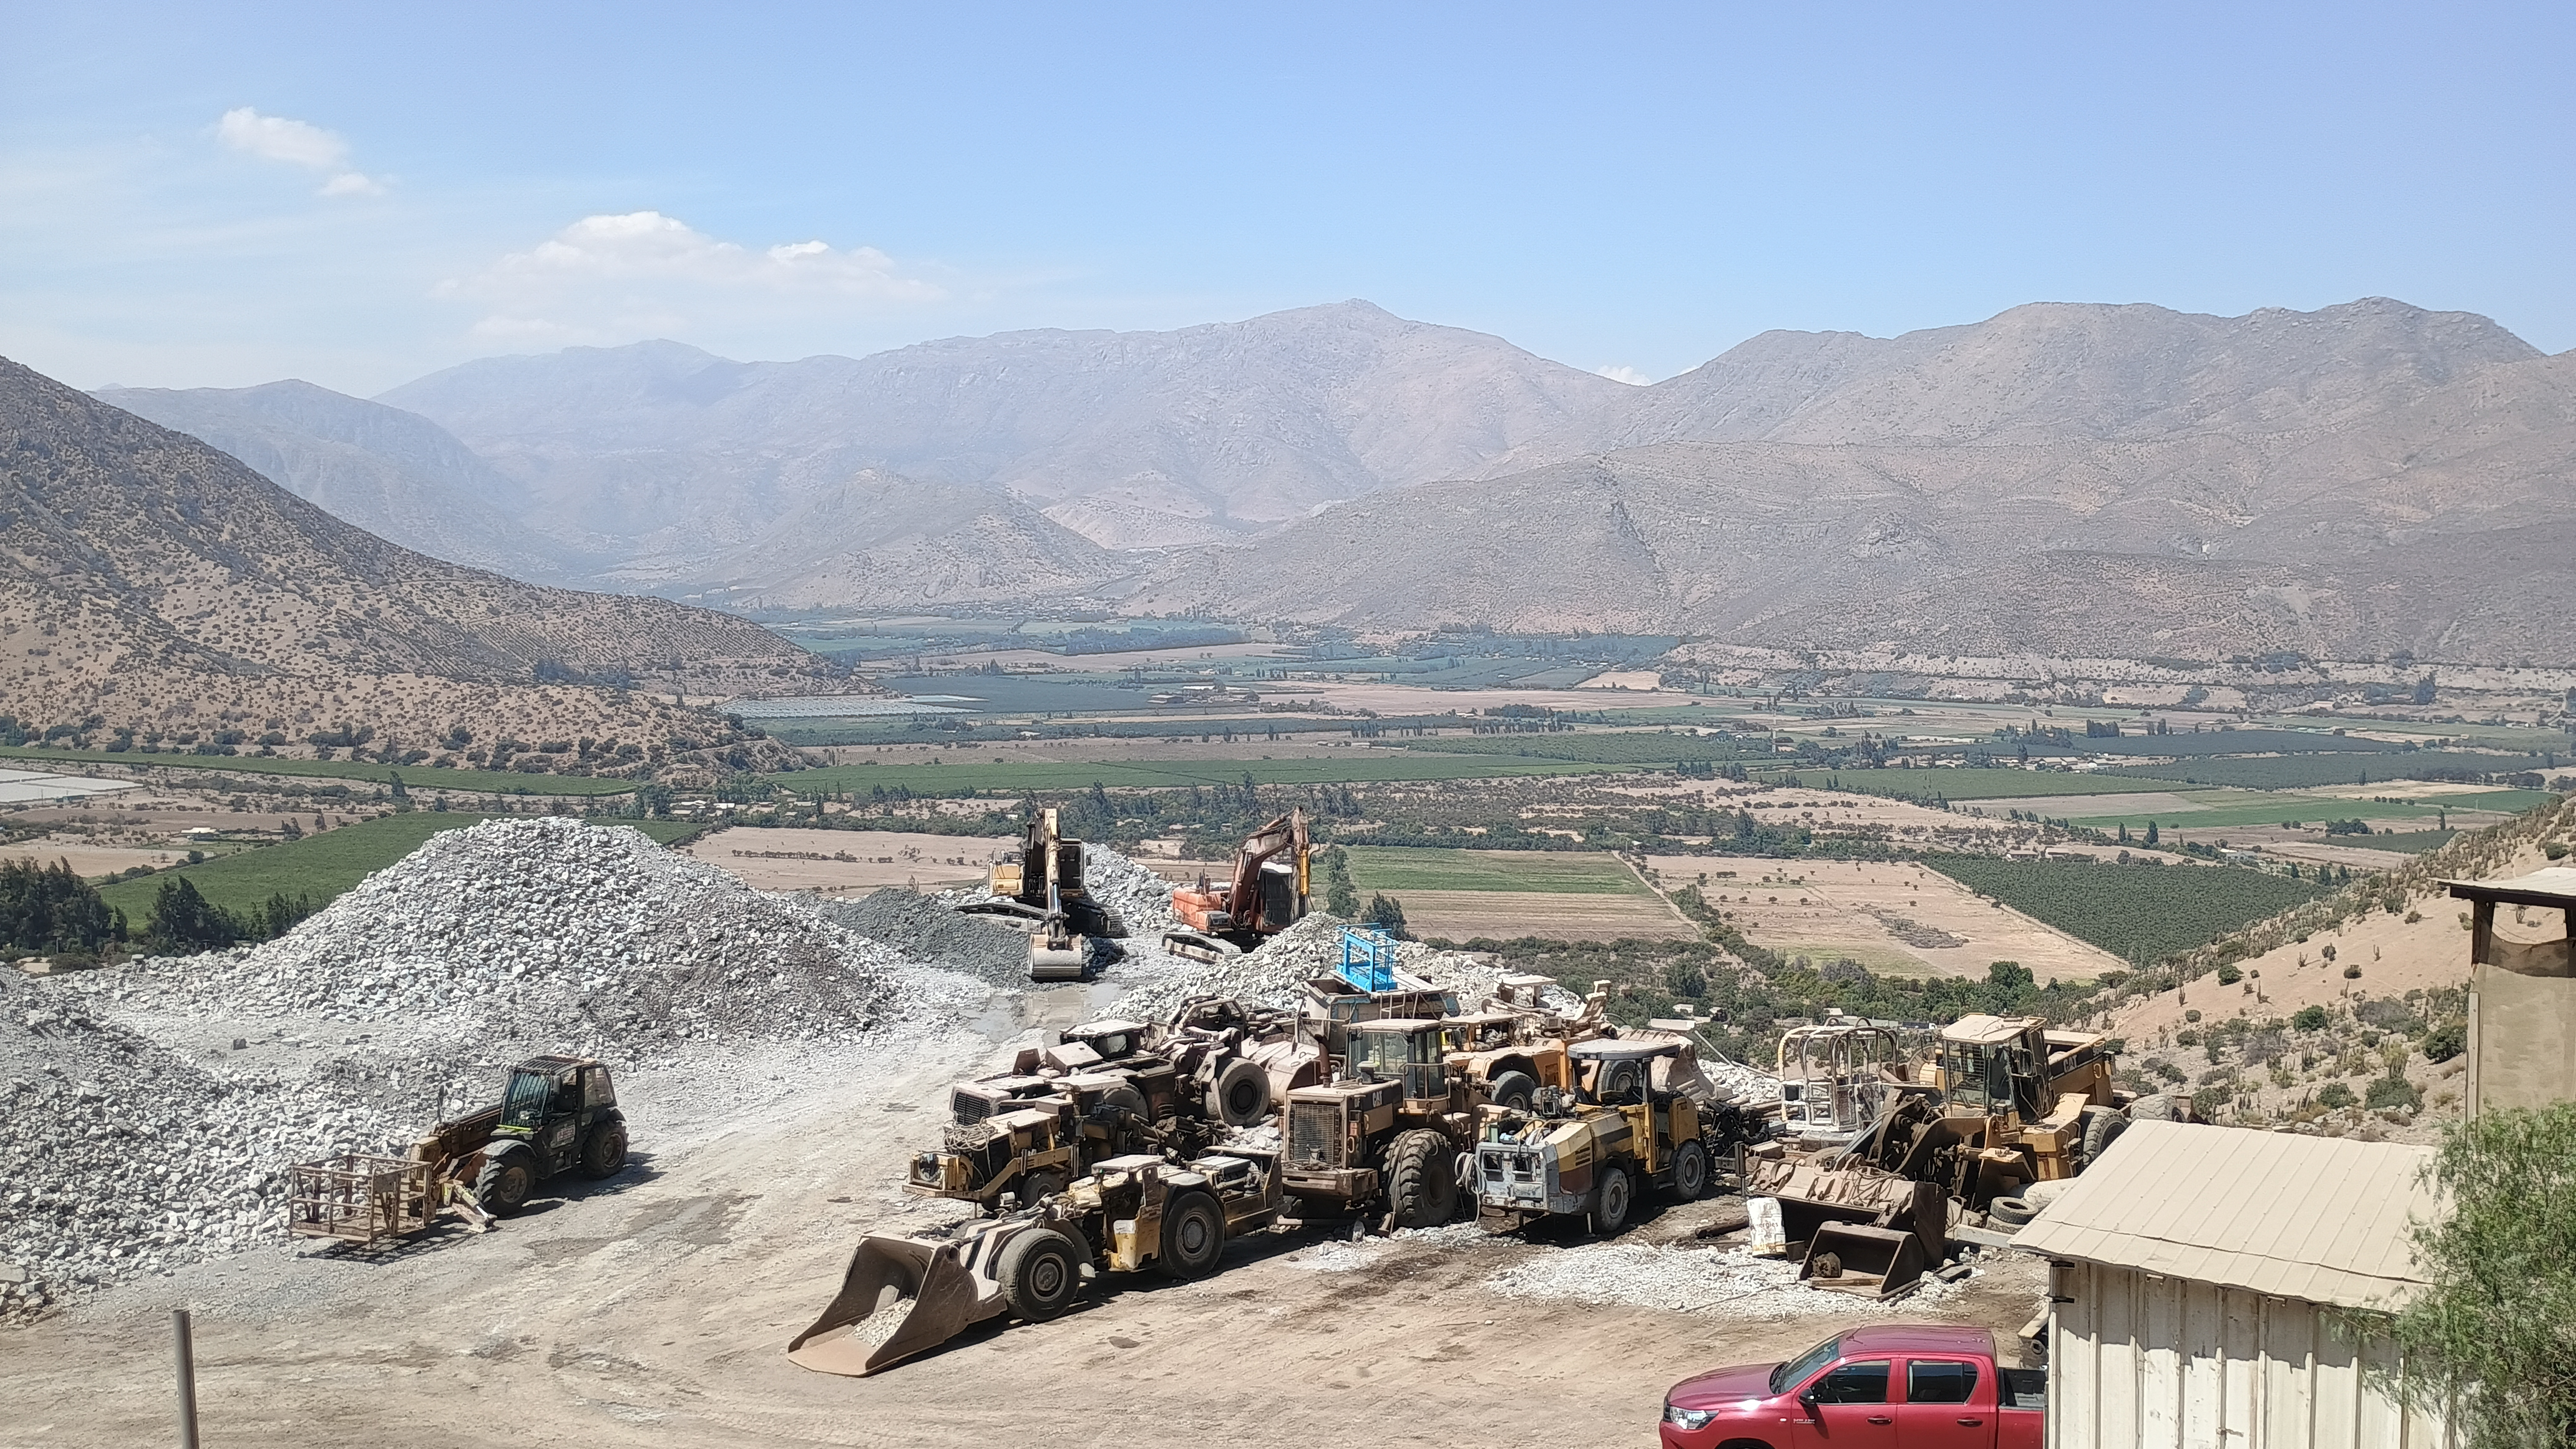
\includegraphics[width=0.7\textwidth]{img/mina/Catemu.jpg}
    \caption{$``Mina$ $Benjamin"$ in Catemu, V Region,Chile.}
    \label{fig:mine}
\end{figure}
\newp
The system was tested in four diferent communication lines, with distances between 15 and 120 meters, proving their capability horizontally and vertically. The test was the following:

\begin{itemize}
    \item Line of 15m: The Transmitter was located at the entrance of the mine, and the receiver with line of sight at 15 meters in. This test was made to prove the basic operation of the system after the trip.
    \newp
    As result the system was able to comunicate with a SER of 0\% and a SNR of 48 dB.

    \begin{figure}[H]
        \centering
        \begin{subfigure}[b]{0.49\textwidth}
            \centering
            \includegraphics[width=\textwidth]{img/mina/Entrada.png}
            \caption{Node at the entrance of the mine.}
            \label{fig:15m_setup}
        \end{subfigure}
        \hfill
        \begin{subfigure}[b]{0.49\textwidth}
            \centering
            \includegraphics[width=\textwidth]{img/mina/SNR ENTRADA.png}
            \caption{Noise and Tone for SNR Measurement.}
            \label{fig:15m_SNR}
        \end{subfigure}
        \caption{Results obtained at 15m distance in the mine.}
        \label{fig:15m-results}
    \end{figure}

    \item Line of 14m: The transmitter was located at a certain mining mantle and the receiver in another mining mantle at a distance of 40m directly Through rock. This was the already a valuable measurement due to these two mantles are incommunicated. As result the system was able to communicate with a SER of 0\% and a SNR of 26 dB.
    
    \begin{figure}
        \centering
        \begin{subfigure}[b]{0.49\textwidth}
            \centering
            \includegraphics[width=\textwidth]{img/mina/Manto 1 setup.png}
            \caption{Node at the mining mantle.}
            \label{fig:40m_setup}
        \end{subfigure}
        \hfill
        \begin{subfigure}[b]{0.49\textwidth}
            \centering
            \includegraphics[width=\textwidth]{img/mina/SNR MANTO 1.png}
            \caption{Noise and Tone for SNR Measurement.}
            \label{fig:40m_SNR}
        \end{subfigure}
        \caption{Results obtained at 40m distance in the mine.}
        \label{fig:40m-results}
    \end{figure}

    Additionally here are some correlation forms of detection process at this distance:

    \begin{figure}[H]
        \centering
        \includegraphics[width=0.7\textwidth]{img/mina/corrs Manto 1.png}
        \caption{Correlation form at 40m distance in the mine.}
        \label{fig:40m-corr}
    \end{figure}
    
    \item Line of 20m: The transmitter was located at a tunnel in superior level and the receiver in a tunnel in an deep level, with a distance of 20m. This was the first vertical communication test. As result the system was able to communicate with a SER of 0\% and a SNR of 37 dB.
    
    \begin{figure}
        \centering
        \begin{subfigure}[b]{0.49\textwidth}
            \centering
            \includegraphics[width=\textwidth]{img/mina/Nivel sup Setup.png}
            \caption{Node at the superior tunnel.}
            \label{fig:20m_setup}
        \end{subfigure}
        \hfill
        \begin{subfigure}[b]{0.49\textwidth}
            \centering
            \includegraphics[width=\textwidth]{img/mina/SNR sup 1.png}
            \caption{Noise and Tone for SNR Measurement.}
            \label{fig:20m_SNR}
        \end{subfigure}
        \caption{Results obtained at 20m distance in the mine.}
        \label{fig:20m-results}
    \end{figure}
    
    \item Line of 120m: The transmitter was located deep in mine at surface level and the receiver was located outside the mine, near of the offices, with a distance of 120m. This was the longest communication test. As result the system was able to communicate with an average SER of 0.35\%
    %%Revisar, debo calcular SER para cada test en solitario
    and a SNR of -9 dB.

    \begin{figure}
        \centering
        \begin{subfigure}[b]{0.49\textwidth}
            \centering
            \includegraphics[width=\textwidth]{img/mina/setup refugio.jpeg}
            \caption{Node at the surface level inside the mine.}
            \label{fig:120m_setup}
        \end{subfigure}
        \hfill
        \begin{subfigure}[b]{0.49\textwidth}
            \centering
            \includegraphics[width=\textwidth]{img/mina/SNR 120m.png}
            \caption{Noise and Tone for SNR Measurement.}
            \label{fig:120m_SNR}
        \end{subfigure}
        \caption{Results obtained at 120m distance in the mine.}
        \label{fig:120m-results}
        \end{figure}
    Additionally here are some correlation forms of detection process at this distance:

    \begin{figure}[H]
        \centering
        \includegraphics[width=0.7\textwidth]{img/mina/corrs 120 m.png}
        \caption{Correlation forms at 120m distance in the mine.}
        \label{fig:120m-corr}
    \end{figure}
\end{itemize}

\section{Results Summary}
